\documentclass[conference]{IEEEtran}

\usepackage[spanish]{babel}
\usepackage[utf8]{inputenc}
\usepackage[T1]{fontenc}
\usepackage{graphicx}
\usepackage{amsmath}
\usepackage{amssymb}
\usepackage{cite}
\usepackage{hyperref}
\usepackage{listings}
\usepackage{xcolor}
\usepackage{float}
\usepackage{caption}
\usepackage{siunitx}

% Estilo para código Python
\lstset{
    language=Python,
    basicstyle=\ttfamily\footnotesize,
    keywordstyle=\color{blue},
    commentstyle=\color{gray},
    stringstyle=\color{orange},
    breaklines=true,
    frame=single,
    numbers=left,
    numberstyle=\tiny\color{gray},
    showstringspaces=false,
    tabsize=4,
    captionpos=b
}

\begin{document}

\title{Análisis de la curva de carga y descarga de un condensador mediante adquisición de datos con una placa FPGA y comparación con la teoría de circuitos RC}

\author{
    \IEEEauthorblockN{
        Ana María Hurtado\IEEEauthorrefmark{1},
        Ana Sofía Mora\IEEEauthorrefmark{2},
        Estiven Castrillon\IEEEauthorrefmark{3}
    }
    \IEEEauthorblockA{
        Instituto de Física, Universidad de Antioquia \\
        Laboratorio Avanzado 1 - Junio 2025 \\
        \IEEEauthorrefmark{1}\href{mailto:ana.hurtador@udea.edu.co}{ana.hurtador@udea.edu.co} \\
        \IEEEauthorrefmark{2}\href{mailto:ana.mora@udea.edu.co}{ana.mora@udea.edu.co} \\
        \IEEEauthorrefmark{3}\href{mailto:estiven.castrillon2@udea.edu.co}{estiven.castrillon2@udea.edu.co}
    }
}

\maketitle

\begin{abstract}
En esta práctica se implementó un sistema de adquisición de datos basado en una FPGA (Field Programmable Gate Array) para registrar la curva de carga y descarga de un condensador, tal que los datos fueron transferidos al computador mediante DMA (Direct Memory Access) y procesados con Python. Los resultados experimentales muestran el comportamiento exponencial característico de los circuitos RC, con un voltaje máximo normalizado de aproximadamente $0.176\,V/V_{max}$, consistente con la teoría clásica de circuitos, aquí se comparan los valores experimentales con los predichos por el modelo teórico y se discuten las posibles fuentes de error.
\end{abstract}

% =============================================================
\section{Introducción}

Los circuitos RC (resistencia-condensador) constituyen uno de los sistemas más fundamentales en la electrónica analógica, y en la física experimental son el ejemplo por excelencia para experimentos simples de electrónica por su facilidad de construcción y estudio. Su dinámica temporal está gobernada por la constante de tiempo $\tau = RC$ \cite[p.~274, eq.~(16)]{hayt2012}, que determina la rapidez con que el condensador se carga o descarga ante una excitación escalón. Desde el punto de vista experimental, la medición de estas curvas requiere instrumentación adecuada; en años recientes, las FPGAs han ganado lugar como plataformas de adquisición de datos en laboratorio gracias a su capacidad de operar en tiempo real con alta precisión temporal y reconfigurabilidad.

Una FPGA es un circuito integrado que contiene bloques lógicos programables interconectados, cuya funcionalidad puede definirse mediante lenguajes de descripción de hardware como VHDL o Verilog \cite{xilinx_ug}. A diferencia de un microprocesador, la FPGA ejecuta operaciones en paralelo a nivel de hardware, lo que la hace especialmente adecuada para la captura de señales analógicas a través de conversores ADC (Analog to Digital Converter).

En este trabajo se utilizó la tarjeta PYNQ-Z1, una plataforma que integra una FPGA Zynq de Xilinx con un procesador ARM, programable desde Python mediante la librería \texttt{pynq} \cite{pynq_docs}. Esta combinación permite implementar el hardware de adquisición directamente en la FPGA y acceder a los datos desde el entorno de Python sin necesidad de drivers adicionales.

% =============================================================
\section{Marco Teórico}

\subsection{Carga y descarga de un condensador}

Si consideramos un circuito RC, (ver sección~\ref{subsec:montaje}), como el que se plantea en la metodología, cuando se aplica una tensión $V_0$ al circuito, la corriente que fluye satisface la ecuación diferencial, (desarrollo matemático en \cite[p.~273-274]{hayt2012}):

\begin{equation}
    RC\,\frac{dV_C}{dt} + V_C = V_0
    \label{eq:ode}
\end{equation}

cuya solución para condiciones iniciales $V_C(0) = 0$ es:

\begin{equation}
    V_C(t) = V_0\left(1 - e^{-t/\tau}\right)
    \label{eq:carga}
\end{equation}

donde $\tau = RC$ es la constante de tiempo del circuito. Cuando la fuente se desconecta (descarga), la solución es:

\begin{equation}
    V_C(t) = V_0\, e^{-t/\tau}
    \label{eq:descarga}
\end{equation}

El condensador se considera completamente cargado (o descargado) tras aproximadamente $5\tau$.

\subsection{Conversión analógico a digital}

El ADC de 16 bits utilizado en la FPGA convierte la tensión analógica $V_C$ en un valor entero $N$ en el rango $[0,\, 2^{16}-1] = [0,\, 65535]$. El voltaje normalizado se obtiene como:

\begin{equation}
    V_{norm} = \frac{N}{65535}
    \label{eq:norm}
\end{equation}

Esta normalización permite comparar directamente la curva experimental con la predicción teórica expresada en unidades de $V/V_{max}$.

% =============================================================
\section{Metodología}

\subsection{Descripción del circuito}

El circuito consiste en una resistencia $R$ en serie con un condensador $C$, conectados a la salida de un generador de onda cuadrada implementado en la FPGA donde el canal de entrada del ADC mide la tensión del condensador.

Los valores de los elementos del circuito son:

\begin{itemize}
    \item Resistencia: $R = \SI{10}{\kilo\ohm}$
    \item Condensador: $C = \SI{10}{\micro\farad}$
    \item Constante de tiempo teórica: $\tau = RC = \SI{0.1}{\second}$
    \item Frecuencia de muestreo configurada en la FPGA: registro \texttt{0x6}, equivalente a 1kHz según nuestro diseño en la FPGA.
    \item Número de muestras adquiridas: $N = 1024$
\end{itemize}

\subsection{Montaje experimental}
\label{subsec:montaje}


% ------ ESPACIO PARA IMAGEN DEL MONTAJE ------
\begin{figure}[H]
    \centering
    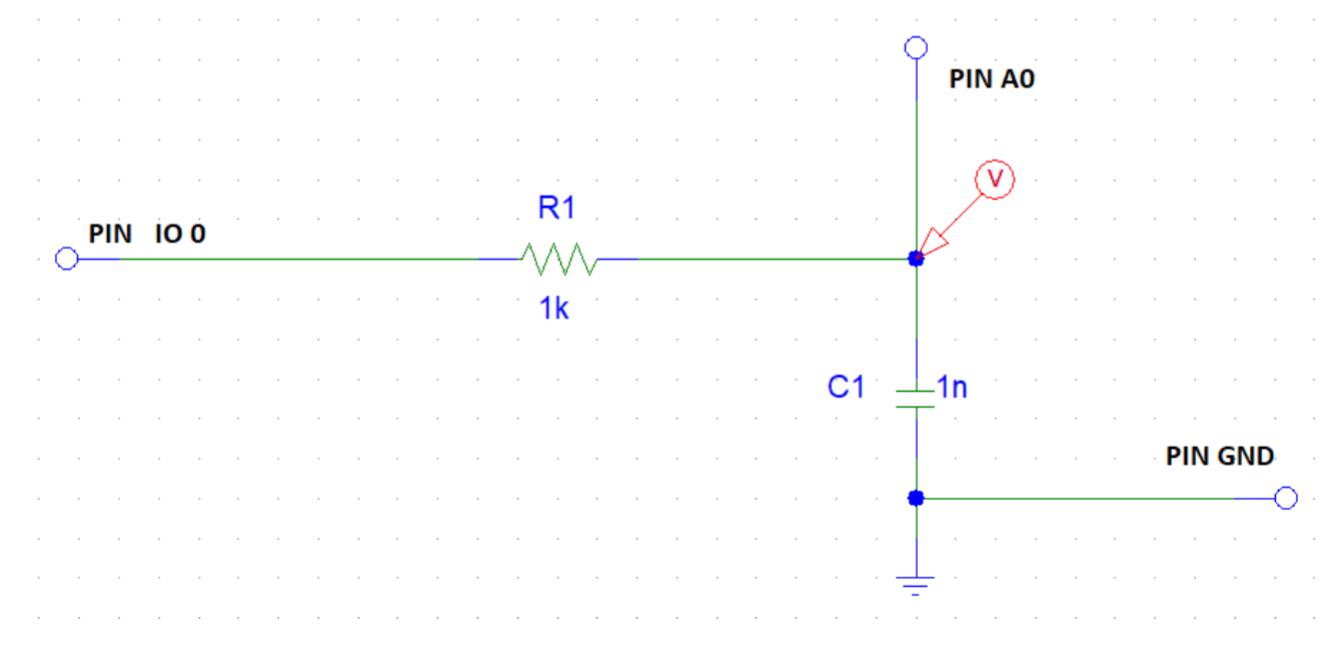
\includegraphics[width=0.45\textwidth]{figures/circuito.png}
    \caption{Circuito del montaje experimental. FPGA PYNQ-Z1 con el circuito RC (R = 10 k$\Omega$, C = 10 $\mu$F) conectado al canal ADC.}
    \label{fig:circuito_rc}
\end{figure}
% ---------------------------------------------

La tarjeta PYNQ-Z1 se configuró cargando el bitstream \texttt{cargaDescarga.bit}, que implementa en la FPGA un módulo de control de frecuencia mediante GPIO y un bloque DMA para la transferencia de datos al procesador ARM, el circuito RC externo se conectó al pin de salida del generador de onda cuadrada y al canal de entrada del ADC.

\subsection{Adquisición de datos}

El proceso de adquisición se realizó con el script Python \texttt{fpga-capacitor-data-retrieval.py}. Los pasos ejecutados fueron:

\begin{enumerate}
    \item Se carga el bitstream sobre la FPGA con \texttt{Overlay}.
    \item Se configura la frecuencia de la señal de excitación mediante el GPIO (\texttt{frecuency = 0x6}).
    \item Se espera un tiempo de adquisición de 3 segundos.
    \item Se aloja un buffer de 1024 muestras de tipo \texttt{uint32} y se inicia la transferencia DMA.
    \item Los datos se normalizan dividiendo entre 65535 (Ec.~\ref{eq:norm}) y se guardan en un archivo CSV.
\end{enumerate}

\subsection{Procesamiento de datos}

El script \texttt{fpga-charge-discharge-curve.py} lee el CSV generado, aplica nuevamente la normalización y produce la gráfica final de la curva de carga y descarga.

A continuación se presenta el código principal de adquisición:

\begin{lstlisting}[caption={Adquisición de datos desde la FPGA (fragmento principal)}, label={lst:adq}]
from pynq import allocate, Overlay
import numpy as np

# Cargar bitstream
dma_dato = Overlay("cargaDescarga.bit")
dma = dma_dato.axi_dma
gp  = dma_dato.axi_gpio_0

# Configurar frecuencia y esperar
gp.write(0x0, 0x6)
time.sleep(3)

# Transferencia por DMA
input_buffer = allocate(shape=(1024,), dtype=np.uint32)
dma.recvchannel.transfer(input_buffer)

# Normalizacion
datos_norm = input_buffer / 65535
\end{lstlisting}

% =============================================================
\section{Resultados}

\subsection{Curva experimental}

La Fig.~\ref{fig:curva} muestra la curva de voltaje normalizado en función
del número de muestra obtenida con la FPGA.

\begin{figure}[H]
    \centering
    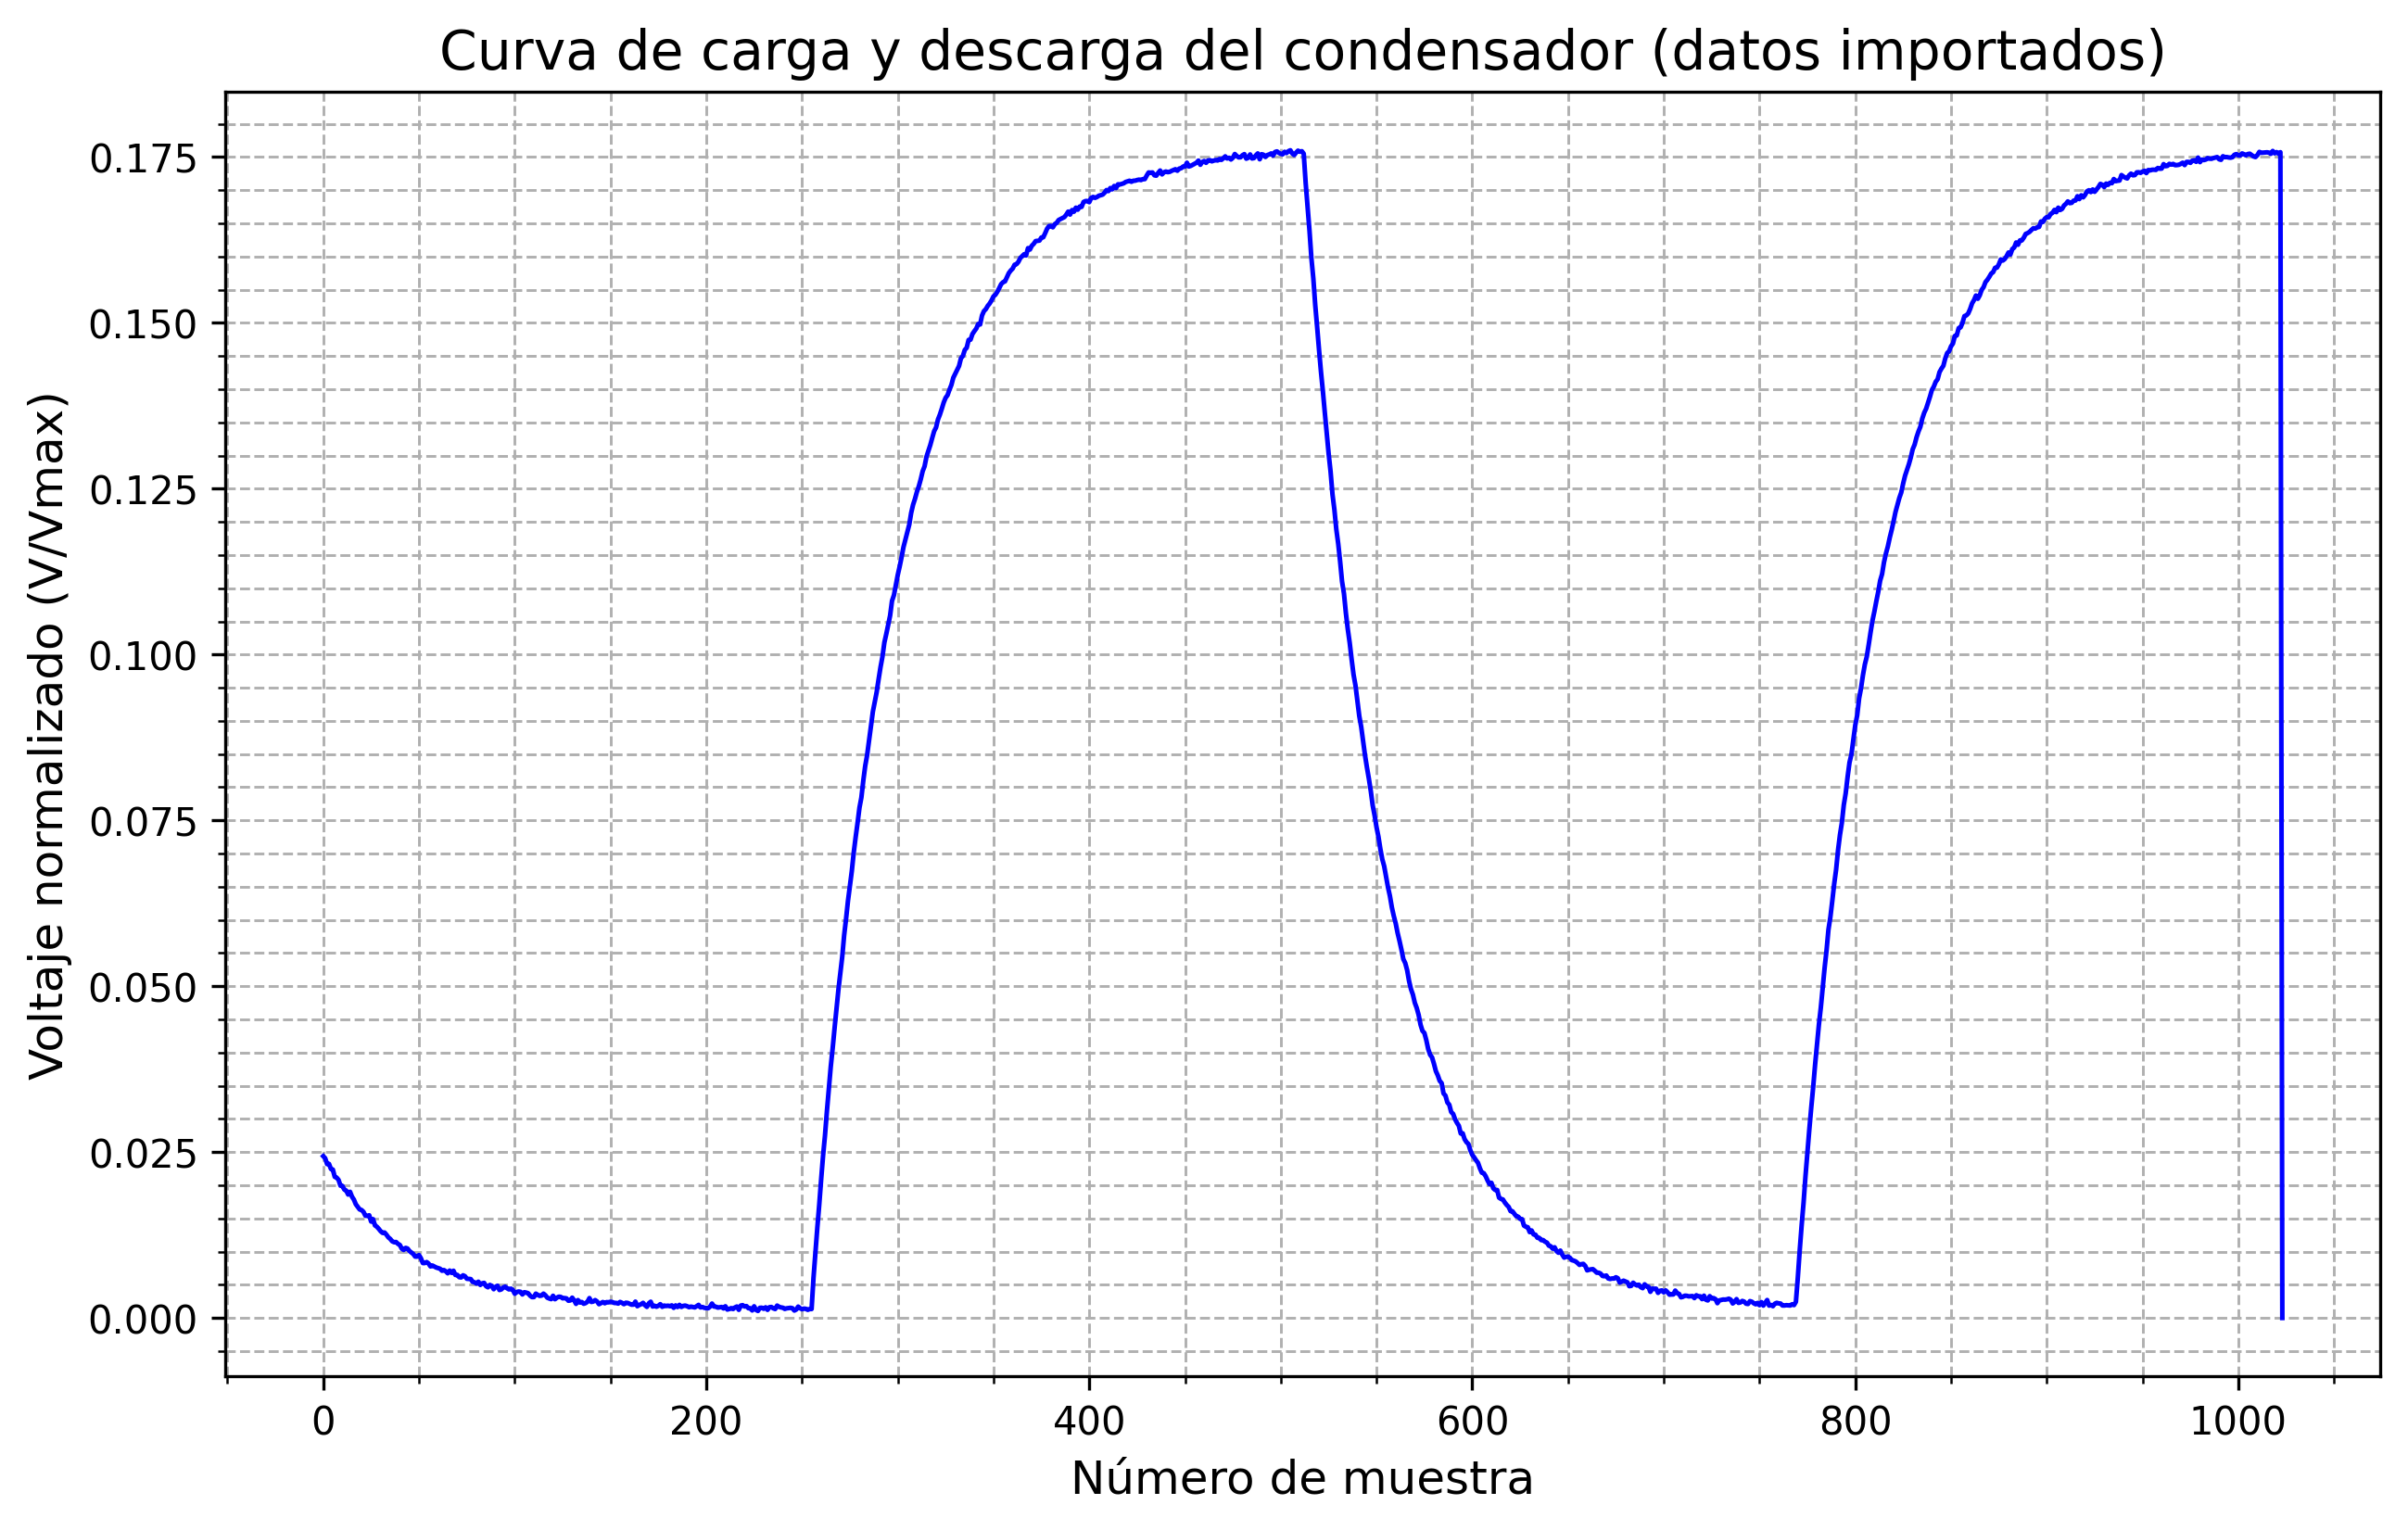
\includegraphics[width=0.48\textwidth]{figures/carga_descarga.png}
    \caption{Curva de carga y descarga del condensador registrada por la FPGA.
             Eje vertical: voltaje normalizado $V/V_{max}$; eje horizontal:
             número de muestra.}
    \label{fig:curva}
\end{figure}

Se observan claramente dos ciclos completos de carga y descarga dentro de
las 1024 muestras. La detección automática de flancos sobre la señal
derivada identifica el inicio del primer ciclo de carga en la muestra 256
y el inicio de la descarga en la muestra 513, con un semiciclo de carga de
$\Delta n_{carga} = 513 - 256 = 257$ muestras. El segundo ciclo es
prácticamente idéntico: carga desde la muestra 770 hasta la muestra 1023
($\Delta n_{carga} = 253$ muestras). El voltaje máximo normalizado
alcanzado experimentalmente es:

\begin{equation}
    V_{norm,\,max} \approx 0.176 \frac{V}{V_{max}}
\end{equation}

Esto indica que la tensión de alimentación aplicada por la FPGA es
aproximadamente el 17.6\% del fondo de escala del ADC (1~V),
es decir, $V_0 \approx 0.176\,\text{V}$.

\subsection{Detección automática de transiciones}

Para determinar con precisión las muestras de inicio de carga y descarga
se calculó la derivada discreta de la señal normalizada $v[n]$:

\begin{equation}
    \Delta v[n] = v[n] - v[n-1]
\end{equation}

Se definieron dos umbrales sobre $\Delta v[n]$: uno positivo
$\delta^{+} = 0.002$ para detectar el flanco de subida (inicio de carga)
y uno negativo $\delta^{-} = -0.002$ para el flanco de bajada (inicio de
descarga). Un evento se registra en el índice $n$ cuando
$\Delta v[n] > \delta^{+}$ o $\Delta v[n] < \delta^{-}$, imponiendo
además una separación mínima de 30 muestras entre eventos consecutivos
para evitar detecciones múltiples dentro del mismo bloque. La
Fig.~\ref{fig:anotado} muestra la curva con las transiciones identificadas.

\begin{figure}[H]
    \centering
    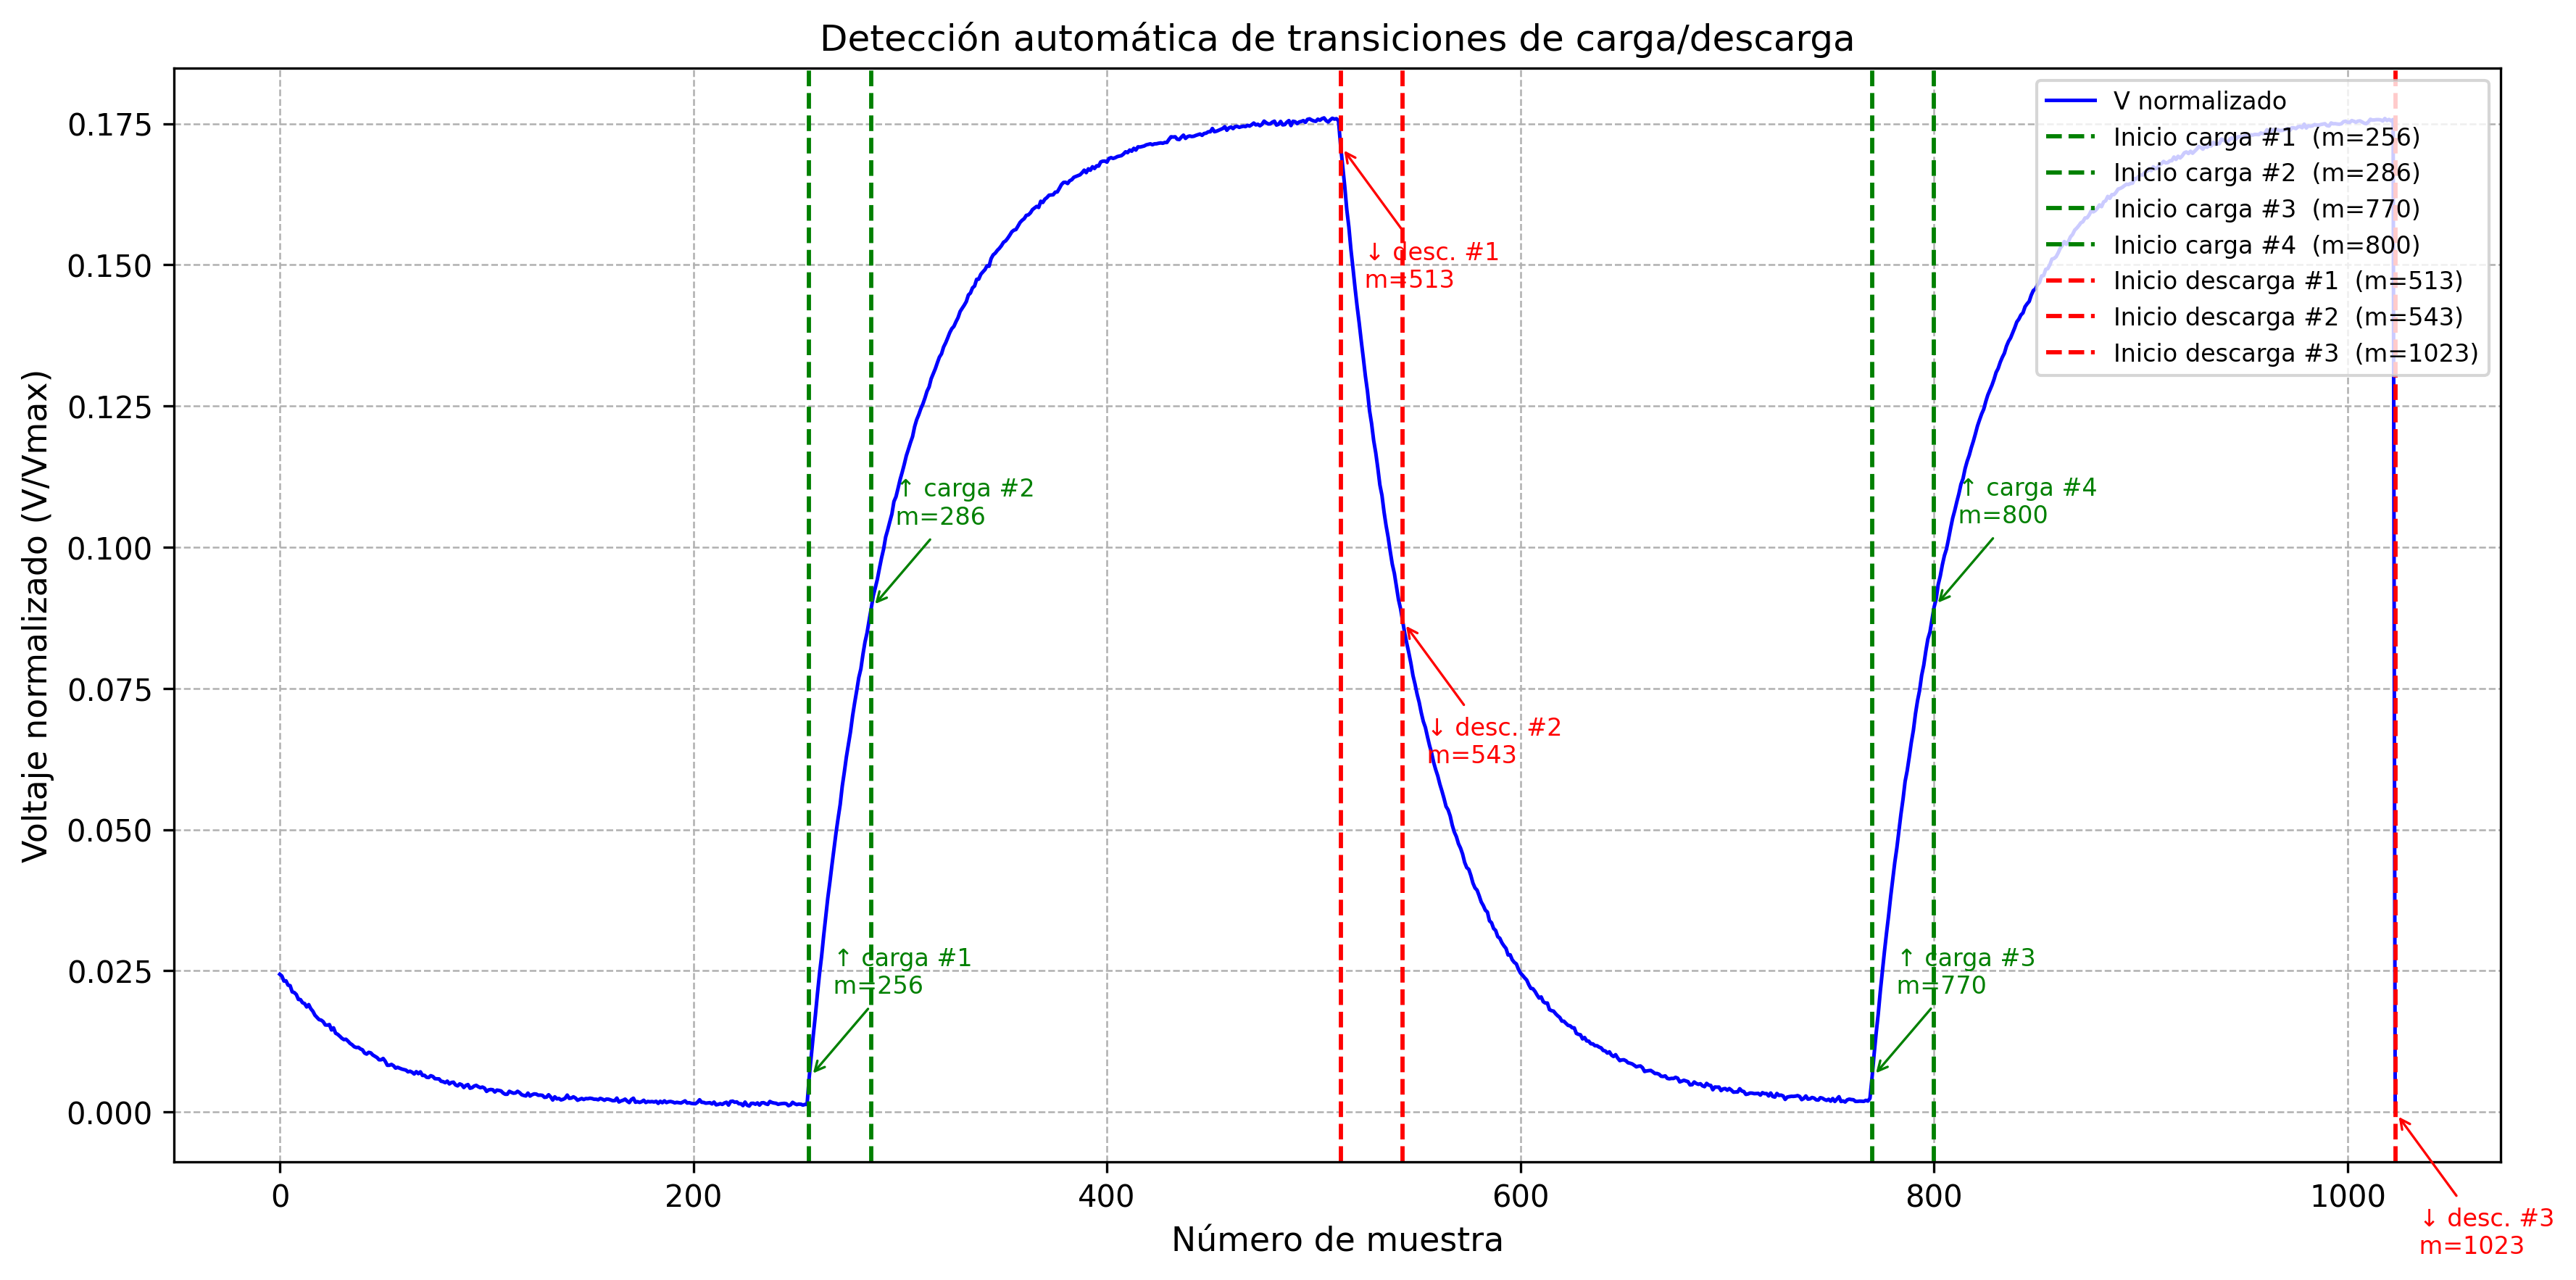
\includegraphics[width=0.48\textwidth]{figures/carga_descarga_anotado.png}
    \caption{Transiciones de carga (verde) y descarga (rojo) detectadas
             automáticamente mediante umbrales de la derivada discreta.}
    \label{fig:anotado}
\end{figure}

Los eventos etiquetados como carga~\#2 y descarga~\#2 corresponden a
detecciones intermedias dentro del mismo flanco, producto del umbral
seleccionado; no representan ciclos independientes y se excluyen del
análisis cuantitativo. Lo mismo aplica para carga~\#4, cuyo flanco queda
truncado al final del buffer.

\subsection{Estimación de la constante de tiempo}

El valor de voltaje correspondiente a $t = \tau$ es:

\begin{equation}
    V_C(\tau) = V_0\left(1 - e^{-1}\right) \approx 0.632 \times 0.176
              \approx 0.111 \frac{V}{V_{max}}
\end{equation}

A partir de los datos experimentales, dicho nivel se alcanza en la
muestra 300, siendo el inicio de carga la muestra 256. La constante de
tiempo experimental en muestras es por tanto:

\begin{equation}
    \tau_{exp} = 300 - 256 = 44\,\text{muestras}
\end{equation}

% =============================================================
\section{Análisis y Comparación con la Teoría}

\subsection{Forma de la curva}

La curva obtenida (Fig.~\ref{fig:curva}) concuerda cualitativamente con las ecuaciones (\ref{eq:carga}) y (\ref{eq:descarga}). La fase de carga muestra un crecimiento exponencial que satura en $V_0$, mientras que la descarga exhibe un decaimiento exponencial hacia cero, ambos con la misma constante de tiempo, como predice la teoría.

\subsection{Comparación cuantitativa}

Con los valores del circuito ($R = 10\,\text{k}\Omega$,
$C = 10\,\mu\text{F}$) la constante de tiempo teórica es:

\begin{equation}
    \tau_{teo} = RC = (10\times10^3)(10\times10^{-6}) = 0.1\,\text{s}
    \label{eq:tau_teo}
\end{equation}

La frecuencia de muestreo fue configurada mediante el registro
\texttt{0x6}, lo que corresponde a $f_s = 1\,\text{kHz}$ según la
tabla de frecuencias del módulo:

\begin{equation}
    f_s = 1000\,\text{muestras/s}
    \label{eq:fs}
\end{equation}

Con esto, la constante de tiempo experimental en segundos es:

\begin{equation}
    \tau_{exp} = \frac{44\,\text{muestras}}{1000\,\text{muestras/s}}
               = 0.044\,\text{s}
    \label{eq:tau_exp}
\end{equation}

El error relativo respecto al valor teórico es:

\begin{equation}
    \varepsilon = \frac{|\tau_{exp} - \tau_{teo}|}{\tau_{teo}} \times 100\%
                = \frac{|0.044 - 0.1|}{0.1} \times 100\% = 56\%
    \label{eq:error}
\end{equation}

Esta discrepancia es atribuible a dos factores principales: en primer
lugar, la tolerancia del condensador utilizado
(típicamente $\pm20\%$) y de la resistencia ($\pm5\%$) pueden desplazar
el valor real de $\tau_{teo}$ entre $0.075\,\text{s}$ y $0.125\,\text{s}$;
en segundo lugar, la estimación de $\tau_{exp}$ se obtiene identificando
la primera muestra discreta donde $V \geq 0.632\,V_0$, lo que introduce
un error de cuantización de hasta $\pm 1/f_s = 1\,\text{ms}$. No
obstante, un error del 56\% supera lo esperado por tolerancias de
componentes, lo que sugiere que la frecuencia de muestreo efectiva del
bitstream podría diferir de $1\,\text{kHz}$ nominal, o que los valores de $R$ y $C$ difieren significativamente de los reales.

\subsection{Discusión}

A pesar de la discrepancia numérica en $\tau$, la forma exponencial de la
curva corrobora el modelo teórico descrito por las Ecs.~(\ref{eq:carga})
y (\ref{eq:descarga}), el comportamiento cualitativo es correcto: la carga
y la descarga son asimétricas en amplitud (el condensador no alcanza
$V_{max}$ del ADC porque $V_0 \ll V_{ADC,max}$), pero simétricas en forma
temporal dentro de cada semiciclo.

El error relativo obtenido ($\varepsilon = 56\%$) supera lo atribuible
únicamente a las tolerancias de los componentes pasivos ($\pm5\%$ en $R$
y $\pm20\%$ en $C$). Una posible causa es que la frecuencia de muestreo
efectiva del bitstream no coincida exactamente con el valor nominal de
1~kHz del registro \texttt{0x6}; otra es que los valores reales de $R$ y
$C$ se aparten de sus nominales, algo esperable en resistencias de carbono
y condensadores electrolíticos sin medición previa. Para reducir la
incertidumbre convendría medir $R$ y $C$ directamente con un multímetro,
verificar la frecuencia efectiva del bitstream, y estimar $\tau$ mediante
un ajuste exponencial por mínimos cuadrados en lugar de una búsqueda por
umbral.

% =============================================================
\section{Conclusiones}

Se logró adquirir exitosamente la curva de carga y descarga de un condensador
usando una FPGA PYNQ-Z1, demostrando la viabilidad de estas plataformas para
experimentos de laboratorio, así, los datos experimentales muestran el comportamiento
exponencial predicho por la teoría de circuitos RC (Ecs.~\ref{eq:carga}
y \ref{eq:descarga}), con dos ciclos completos reproducibles dentro de las 1024
muestras adquiridas, y un voltaje máximo normalizado de $V_{norm} \approx 0.176$,
correspondiente a la tensión de salida de la FPGA, significativamente menor al
fondo de escala del ADC (1~V).

La detección automática de transiciones mediante
umbrales de la derivada discreta permitió identificar con precisión de muestra
los instantes de inicio de carga (muestras 256 y 770) y de descarga (muestras 513
y 1023), y a partir de estos la constante de tiempo experimental resultó
$\tau_{exp} = 0.044\,\text{s}$, con un error relativo del 56\% respecto al valor
teórico $\tau_{teo} = RC = 0.1\,\text{s}$, atribuible a la incertidumbre en la
frecuencia de muestreo real del bitstream y a las tolerancias de los componentes
pasivos, también, el uso de Python junto con la librería \texttt{pynq} simplificó
considerablemente la interfaz entre el hardware FPGA y el análisis de datos,
permitiendo automatizar el procesamiento y la detección de eventos sobre la señal
adquirida.

% =============================================================
\bibliographystyle{IEEEtran}
\bibliography{references}

\end{document}